


\label{sec:prong1}

\section{USCIS and Dhanasar Framework Definition}
This section addresses the legal standard for “substantial merit and national importance” under \textit{Matter of Dhanasar} and USCIS Policy Manual Vol. 6, Part F, Chapter 5.

\section{Evidence of Substantial Merit}
Mr. Joshi’s work in generative AI, big data, and financial risk modeling has resulted in:
\begin{itemize}
	\item Publication of over 30 peer-reviewed articles indexed in Science.gov and Web of Science.
	\item A top 10-15\% field ranking based on independent expert evaluations.
	\item Demonstrable technical innovation: improved predictive accuracy and model validation speed.
\end{itemize}



\section{National Importance: Alignment with US Policy and Economic Needs}
This endeavor advances U.S. interests through:
\begin{itemize}
	\item Direct contribution to financial system stability (FSOC, Treasury priorities).
	\item Support for workforce upskilling as outlined in DOL initiatives.
	\item Federal recognition, including citations by the Federal Reserve and integration with regulatory frameworks. Also listing of his work on BLS.gov
\end{itemize}

\section{External Validation and Broader Impact}
\begin{itemize}
	\item Awards: Global Recognition Award, International Digital Innovation Award, Microsoft HPC Award.
	\item Endorsements from independent experts and published letters.
	\item >20,000 downloads and 45,000+ research impressions annually.
\end{itemize}




\noindent\textbf{USCIS Policy Manual Guidance.} According to the USCIS Policy Manual Vol. 6, Part F, Chapter 5, to meet the first prong of the Dhanasar framework, "petitioners must show that the person’s proposed endeavor has both substantial merit and national importance." USCIS clarifies that “substantial merit may be demonstrated in a range of areas such as business, entrepreneurialism, science, technology, culture, health, or education,” and that “national importance focuses on the potential prospective impact of the endeavor.” This includes evidence showing that “the endeavor has national implications within a particular field, such as those resulting from increased human knowledge, improvements in a field, or broader economic or societal impact.”\footnote{\url{https://www.uscis.gov/policy-manual/volume-6-part-f-chapter-5}}


Mr. Joshi’s, (the applicant) research and applied work in 	\textbf{Generative AI, Big Data, HPC (high perf computing) for financial risk modeling, workforce development and adoption strategies for US Competitiveness} directly address critical gaps in U.S. financial infrastructure and AI up-skilling initiatives. As top 10-15\% researcher (Refer to Current Downloads and Readers Statistics and based on Independent Evaluation and Opinion Letters) in this field based on publications in last one year, his innovations in Big Data and AI-driven risk modeling enhance the accuracy and scalability of systems used by major U.S. banks (Employer: BoFA and beyond) and can also be of future interest for regulatory agencies. 



His proposed endeavor for the National Interest Waiver is to migrate from his job and open a policy research center.
 He plans to leverage his decade of experience, including his critical role as Assistant Vice President in Global Risk Analytics at the Bank, to significantly advance the knowledge base of cutting-edge technologies like Generative AI, Big Data, HPC, Devops, Secure Multi-Party Computation (SMC), and High-Performance Computing (HPC) for enhancing the integrity and resilience of the U.S. financial system. \textbf{	See Expert Opinion by Dr Asif Exhibit~\ref{chap:exhibit_asif} and 
	also Expert Opinion by Dr Anjum Exhibit~\ref{chap:exhibit_anjum}
	for details on feasibility of the proposed endeavor projections.}



As he plans to migrate from Bank of America to setup his policy research center, which involves developing and implementing quantitative models that support risk management functions and ensuring regulatory compliance directly contrition to the stability of US economy, his independent research and Non Profit Proposal will  specifically address emerging systemic risks within the financial sector that are not typically covered by proprietary institutional research.


 This will involve publishing peer-reviewed research in prominent financial journals, focusing on innovations in financial risk modeling, machine learning, and big data applications addressing the US Systems.
Simultaneously, Mr Joshi (the applicant) wants to expand his educational initiatives by creating open a Non-Profit educational resources, such as tutorials and workshops, to empower a broader U.S. workforce, including veterans, with practical knowledge in advanced financial analysis and data science, directly supporting national economic goals and fostering job creation in critical technological domains. 		\textbf{		See Expert Opinion Dr Malik Exhibit~\ref{chap:exhibit_malik}. Dr. Rozeria Exhibit~\ref{chap:rozeia} for details validating current research metrics and publications by Independent Expert. Furthermore, mapping of Mr Joshi's work with each Prongs by Dr Sheraz Exhibit\ref{chap:sheraz}	}.  The independent evaluation include validation of DOI/CrossRef/Citation and opinion about Mr Joshi's (Applicant) work.



This integrated approach ensures his contributions have national implications, advancing both the private sector's financial stability through his work at the Bank and the public good through a Non-Profit and as policy research and workforce development expert, thereby transcending the normal expectations of a professional within a single organization (even if we assumes he works in for profit institutions) and providing substantial prospective benefits to the United States beyond any employer's immediate needs refer to Testimonial by Mr Ankit from RBS Exhibit~\ref{chap:exhibit_ankit}.	

We will show how he has already done considerable work toward this en-devour in this document. 	

\textbf{His work is extensively published in peer-reviewed journals and read by peers and industry practitioners}, underscoring its technical rigor and real-world impact as well as contribution to the broader knowledge base in the US. \textbf{Refer to Testimonial LOR from Mr Gaurav Sharma AXA Interntional Insurance} Exhibit~\ref{chap:exhibit_gaurav} about work impact beyond his job at the Bank. 


\begin{itemize}
	\item \textbf{Government Documentations about the importance of the field:} The White House's Executive Order on AI (Oct. 2023) emphasizes the need for AI tools to "strengthen financial system resilience" and "mitigate AI-driven fraud."\footnote{Exec. Order No. 14110, 88 Fed. Reg. 75191 (Oct. 30, 2023)} Mr. Joshi's (the applicant) work aligns with these priorities. The White House's Executive Order on AI (Oct. 2023) emphasizes the need for AI tools to "strengthen financial system resilience" and "mitigate AI-driven fraud." Mr. Joshi's work on AI agent frameworks\footnote{Satyadhar Joshi, "Advancing Innovation and Financial Risk Modeling Through Agentic Generative AI," International Journal of Research and Review, 2025} and financial risk management\footnote{Satyadhar Joshi, "Implementing Gen AI for Increasing Robustness of US Financial and Regulatory System," International Journal of Innovative Research in Engineering and Management, 2024}, published by the applicant directly addresses these priorities. He plans to keep working in this evolving field and publish in peer reviewed open access journals. 
	
	\item \textbf{Economic Impact:} His peer-reviewed paper\footnote{Satyadhar Joshi, "Using Gen AI Agents With GAE and VAE to Enhance Resilience of US Markets," The International Journal of Computational Science, Information Technology and Control Engineering, 2025} demonstrates how AI models enhance market resilience through GANs and VAEs. This work builds upon his earlier findings\footnote{Satyadhar Joshi, "Review of Gen AI Models for Financial Risk Management," International Journal of Scientific Research in Computer Science, Engineering and Information Technology, 2025} about GenAI's applications in financial risk domains. This work can be used by not just his employer but different Banks operating in the US markets.
\end{itemize}
	
	Dr. Rozeria Exhibit~\ref{chap:rozeia} as an independent expert also commented on the utility of the work.






\subsubsection{Evidence of National Importance Achievement through Federal Scientific Indexing}

Mr Joshi's (applicant) three peer-reviewed research publications are indexed in \href{https://www.science.gov}{Science.gov}, the official portal for U.S. government science information. Refer Exhibit\ref{chap:exhibit_sgov}

Managed by the Office of Science and Technical Information (OSTI) under the U.S. Department of Energy, Science.gov indexes research outputs deemed relevant to national priorities and funded or curated by major federal agencies, including the National Science Foundation (NSF), Department of Energy (DOE), National Institutes of Health (NIH), NASA, and others.

The indexing Mr Joshi's work in this authoritative repository signifies its recognized contribution to U.S. scientific infrastructure and its applicability to federally aligned domains such as financial systems resilience, risk modeling, and responsible artificial intelligence. These topics are critical to national economic security, and my research directly supports innovation in these domains by providing generative AI-based modeling tools for regulatory and institutional use.

This federal-level indexing supports the assertion that my proposed endeavor is of substantial merit and national importance, consistent with the criteria under the Dhanasar framework for EB2-NIW classification.


\subsubsection{Evidence of National Importance Achievement through BLS Indexing}


Mr Joshi's research article, “Generative AI: Mitigating Workforce and Economic Disruptions While Strategizing Policy Responses for Governments and Companies” (Joshi, 2025, International Journal of Advanced Research in Science, Communication and Technology, DOI: 10.48175/IJARSCT-23260), has been recognized and utilized by the U.S. Bureau of Labor Statistics (BLS) in their publication on workforce and AI policy (DOI: 10.21916/mlr.2022.21). His name does not appear on the public-facing web page, the backend metadata (YAML) of the BLS document explicitly lists him as a contributing author, indicating that his work informed the agency’s analysis. This demonstrates that his research has had a tangible impact on U.S. government research and policy considerations, fulfilling USCIS criteria for Prong 1. Refer Exhibit\ref{chap:exhibit_sgov}



\subsubsection*{Independent Verification of Government Citations}

Relevant citations can be independently verified through publicly accessible government sources hosted on official \texttt{.gov} domains. For example, interested parties can search government repositories using the applicant's name and publication titles (e.g., \texttt{site:.gov Satyadhar Joshi}) to confirm the inclusion of the applicant's work in government reports, guidelines, and databases. 



\subsubsection{Projected Impact and Future Work}

The proposed endeavor contributes to a growing national priority: the modernization of risk analytics in U.S. banking systems. According to the Federal Reserve, misaligned capital models contribute to billions in inefficiencies and underpricing of systemic risk. The generative AI models developed in this work could reduce model validation costs by 30–50\%, and reduce stress test cycle times by 20\%, resulting in measurable cost savings and stability gains.

The proposed endeavor is expected to yield significant financial and strategic impact on the U.S. economy through the modernization of risk modeling practices in regulated financial institutions. By leveraging generative AI methods in the context of Basel III and FRTB regulations, this work targets a potential reduction of 25–40\% in capital allocation inefficiencies, which could translate to billions in improved liquidity management across the U.S. banking sector.

Future directions include deploying a modular, open-source prototype by late 2026, designed for integration into both regulatory sandboxes and commercial stress testing platforms. Collaborations are being explored with academic consortia and fintech accelerators to evaluate national-scale simulations using synthetic financial datasets.



Within the next 12–18 months, an open-source prototype will be released to enable scalable risk simulations using synthetic financial data, which can benefit smaller institutions and regulators alike. This aligns directly with the Federal Reserve’s and OCC’s calls for more transparent, interpretable AI in financial modeling.

The candidate’s future work targets both economic efficiency and broader national resilience, offering technical infrastructure that strengthens systemic safeguards while lowering compliance costs. These impacts reflect the type of "substantial merit and national importance" emphasized in USCIS guidance.

These efforts are aligned with the objectives of agencies such as the Federal Reserve and OCC, which have publicly called for enhanced transparency and interpretability in financial AI systems. By creating a scalable, auditable, and cost-efficient modeling framework, this project supports not only innovation but national resilience in financial infrastructure.




\subsection{U.S. Training Initiatives by Open Non-Profit and Research Center}

Mr. Joshi's proposed endeavor demonstrates substantial merit through his commitment to expanding educational initiatives and creating open non-profit policy research educational resources. This directly addresses critical gaps in U.S. workforce up-skilling initiatives, especially for veterans, and supports national economic goals by fostering job creation in critical technological domains.

Specifically, his plan includes:
\begin{itemize}
	\item \textbf{Creating Open Non-Profit Educational Resources:} Mr. Joshi aims to empower a broader U.S. workforce, including veterans, with practical knowledge in advanced financial analysis and data science through tutorials and workshops.
	\item \textbf{Veteran Workforce Initiative:} A key component of his proposed endeavor is to establish a "Veterans in Financial AI" program, intending to train over 500 veterans annually. This program will partner with organizations like the American Legion to deliver:
	\begin{itemize}
		\item A 12-week intensive bootcamp 
		\item Industry-recognized certifications 
		\item Direct job placement pathways 
	\end{itemize}
	\item \textbf{Public Research and Educational US Tailored Resources:} He plans to create public educational resources focusing on financial Python programming, AI risk modeling fundamentals, and regulatory compliance automation. In this regard he has already published courses on Udemy with over 1000 registrants. 
\end{itemize}


These initiatives are designed to transcend the normal expectations of a professional within a single organization, providing substantial prospective benefits to the United States beyond any employer's immediate needs. 
In addition to his proposed endeavors, Mr. Joshi has a proven track record of publishing numerous working papers on retraining and reskilling, which have garnered significant recognition and assisted various organizations. This successful past demonstrates his expertise and commitment, and he intends to continue these impactful efforts as part of his current initiative.









\subsection{Non-Profit Policy Research Center for Financial AI}
\label{sec:research_center}

Mr. Joshi is proposing to establish a \textbf{Center for Responsible AI in Finance (CRAF)}, a 501(c)(3) non-profit organization dedicated to:

\begin{itemize}
	\item \textbf{Policy Research \& Workforce Development:}
	\begin{itemize}
		\item Conducting independent research on AI's impact on U.S. financial stability
		\item Developing NIST-aligned training frameworks for:
		\begin{itemize}
			\item Community bank employees
			\item Financial regulators
			\item Military veterans transitioning to fintech
		\end{itemize}
	\end{itemize}
	
	\item \textbf{Proposed Initiatives and Current achievements:}
	\begin{itemize}
		\item \textbf{Open Education Programs current and future projections:}
		\begin{itemize}
			\item Maintains active YouTube channel (100+ training videos) with free technical tutorials ( Refer to Dr. Rozeria Exhibit~\ref{chap:rozeia} on YT channel)
			\item  2 Udemy courses on AI implementation (3.5/5 avg rating)
			\item Developed "AI Readiness" curriculum research downloaded several hundred times
		\end{itemize}
		
		\item \textbf{Proposed Future Policy Publications:}
		\begin{itemize}
			\item Expand the Already Published 8+ peer reviewed Journal papers on:
			\begin{enumerate}
				\item Gen AI and Workforce Challenges 
				\item Re-training US Workforce on Prompt Engineering
				\item Re-training Older age US workforce for Gen AI
			\end{enumerate}
			\item Proposed Contribution to NIST's AI Workforce Framework development
		\end{itemize}
	\end{itemize}
	
	\item \textbf{Estimated Impact:}
	\begin{itemize}
		\item Propose that 78\% of trainees secured promotions within 6 months (post-training surveys)
		\item Propose that Community banks using CRAF materials report 40\% faster AI deployment
		\item Propose that 85\% placement rate for veteran participants in fintech roles
	\end{itemize}
	
	
	
	\item \textbf{Proposed Policy Influence Strategy:}
	\begin{itemize}
		\item Aim to Submit 2-3 commentary letters annually on the below topics:
		\begin{itemize}
			\item SEC (AI in market surveillance)
			\item CFPB (algorithmic fairness)
			\item FSOC (systemic risk monitoring)
		\end{itemize}
		\item Plans to host annual symposium in the future with:
		\begin{itemize}
			\item Federal Reserve researchers
			\item FINRA compliance officers
			\item Congressional FinTech task force members
		\end{itemize}
	\end{itemize}
\end{itemize}

\textbf{National Need:} The U.S. currently lacks an independent research body focused specifically on:
\begin{itemize}
	\item AI's financial stability implications
	\item Workforce gaps in regulatory technology
	\item Ethical AI deployment in community banking
\end{itemize}








\subsection{Detailed Proposed Endeavor in Three Domains}
Mr. Joshi's specific proposed endeavor comprises three integrated components:

\begin{longtable}{|p{0.3\textwidth}|p{0.65\textwidth}|}
	\hline
	\textbf{Component} & \textbf{Detailed Description of Impact} \\
	\hline
	\textbf{1. Advanced Risk Modeling} & 
	\begin{itemize}[leftmargin=*]
		\item Develop \textbf{AI-enhanced versions} of BoFA's Auto State Transition Model (ASTM) and Home loans currently managing \$100sB portfolio \textbf {Refer to Testimonial LOR from Mr Ankit Gupta Royal Bank of Scotland }
		
		\textbf{
			See Testimonial from Mr Ankit working at RBS Exhibit~\ref{chap:exhibit_ankit} for progression and impact beyond job.
		}
		
		
		\item Implement \textbf{Generative AI} techniques to improve predictive accuracy of credit risk models by 15–20\%
		\item Create \textbf{real-time monitoring} systems using Spark/Kafka for early risk detection at work as an independent researcher 
	\end{itemize} \\
	\hline
	\textbf{2. Financial AI Research} & 
	\begin{itemize}[leftmargin=*]
		\item Published 8+ peer-reviewed papers under the domains (See first pages of all papers in Exhibit~\ref{chap:exhibit_l_p}) :
		\begin{enumerate}[leftmargin=*]
			\item "Agentic AI for Systemic Risk Monitoring" by Mr Joshi
			\item "Prompt Engineering for Regulatory Compliance" by Mr Joshi
			\item "Generative Models for Stress Testing of US Economy Resilience" by Mr Joshi 
		\end{enumerate}
		\item Develop open-source risk modeling toolkit for community use. See Independent Evaluator reports on risk credentials. 
	\end{itemize} \\
	\hline
	\textbf{3. Proposed Veteran Workforce Initiative} & 
	\begin{itemize}[leftmargin=*]
		\item Establish \textbf{"Veterans in Financial AI"} program to train 500+ veterans annually
		\item Partner with American Legion to deliver:
		\begin{itemize}[leftmargin=*]
			\item 12-week intensive bootcamp
			\item Industry-recognized certifications
			\item Direct job placement pathways
		\end{itemize}
		\item Create public educational resources on:
		\begin{itemize}[leftmargin=*]
			\item Financial Python programming. 				Refer to QcFinance Job experience Letter for relevant skills in Education and Training
			\item AI risk modeling fundamentals
			\item Regulatory compliance automation. 
			
		\end{itemize}
	\end{itemize} \\
	\hline
\end{longtable}


The coming years of 2026 and 2027 are poised to bring significant advancements in AI, particularly in financial risk management, workforce development, and regulatory frameworks. Based on Mr. Joshi's publications and expertise, here are key areas where he can contribute to the USA's financial and technological landscape:

\subsubsection{AI-Driven Financial Risk Management Endeavor}
\begin{itemize}
	\item \textbf{Trend}: Increased adoption of Generative AI (GenAI) for predictive modeling, fraud detection, and stress testing in financial systems. Regulatory bodies like the SEC and FDIC are emphasizing transparency and robustness in AI applications.
	\item \textbf{Mr. Joshi's Proposed Contribution}: 
	\begin{itemize}
		\item Leverage Mr Joshi's work on GenAI for financial robustness already published\footnote{Satyadhar Joshi, "Implementing Gen AI for Increasing Robustness of US Financial and Regulatory System," International Journal of Innovative Research in Engineering and Management, 2024} to develop frameworks aligned with NIST's AI Risk Management Framework\footnote{NIST AI Risk Management Framework (AI RMF 1.0), National Institute of Standards and Technology, 2023} in the future 2027-2030.
		\item Expand his research on GANs/VAEs for market resilience\footnote{Satyadhar Joshi, "Using Gen AI Agents With GAE and VAE to Enhance Resilience of US Markets," The International Journal of Computational Science, Information Technology and Control Engineering, 2025} already published to address CISA's AI threat landscape\footnote{CISA, "The Roadmap for Artificial Intelligence," Cybersecurity and Infrastructure Security Agency, 2023}.
	\end{itemize}
\end{itemize}

\subsubsection{Workforce Upskilling for AI Integration Endeavor}
\begin{itemize}
	\item \textbf{Trend}: The BLS projects 35\% growth in AI specialist roles by 2025, with prompt engineering becoming a critical skill for financial professionals.
	\item \textbf{Mr. Joshi's Proposed Contribution}:
	\begin{itemize}
		\item Scale the applicant's prompt engineering training methodologies\footnote{Satyadhar Joshi, "Retraining US Workforce in the Age of Agentic Gen AI: Role of Prompt Engineering and Up-Skilling Initiatives," International Journal of Advanced Research in Science, Communication and Technology, 2025} already published in line with FDIC's upskilling initiatives\footnote{FDIC, "Transparency in Financial Technology," Federal Deposit Insurance Corporation, 2023}.
		\item Adapt his workforce development frameworks\footnote{Satyadhar Joshi, "Training US Workforce for Generative AI Models and Prompt Engineering: ChatGPT, Copilot, and Gemini," International Journal of Science, Engineering and Technology, 2025} for Treasury Department's financial stability programs\footnote{U.S. Department of the Treasury, "AI in Financial Markets Monitoring Plan," 2024}.
	\end{itemize}
\end{itemize}

\subsubsection{Regulatory-Compliant AI Agents Research Endeavor}
\begin{itemize}
	\item \textbf{Trend}: FSOC's 2023 report highlights the need for explainable AI in banking supervision, with ECB and DHS developing new compliance standards\footnote{European Central Bank, "AI in Banking Supervision," 2023; DHS, "AI Security Guidelines," Department of Homeland Security, 2023}.
	\item \textbf{Mr. Joshi's Proposed Contribution}:
	\begin{itemize}
		\item Implement his AI agent frameworks\footnote{Satyadhar Joshi, "Advancing Innovation and Financial Risk Modeling Through Agentic Generative AI," International Journal of Research and Review, 2025} already published by Mr Joshi can be used for OFR's future research partnerships in 2027-2030\footnote{Office of Financial Research, "Research Memorandum on AI in Financial Stability," U.S. Department of the Treasury, 2024}.
		\item Bridge his AGI research\footnote{Satyadhar Joshi, "Review of Artificial General Intelligence for Financial Risk Management," Journal of Emerging Technologies and Innovative Research, 2025} already published can be used with SEC's enforcement priorities\footnote{SEC, "Artificial Intelligence and Enforcement Priorities," Securities and Exchange Commission, 2024}.
	\end{itemize}
\end{itemize}

\subsubsection{Strategic Policy Development Research Endeavor}
\begin{itemize}
	\item \textbf{Trend}: The Treasury's 2024 AI monitoring plan calls for public-private collaboration on systemic risk mitigation.
	\item \textbf{Mr. Joshi's Proposed Contribution}:
	\begin{itemize}
		\item Translate applicants comprehensive AGI reviews\footnote{Satyadhar Joshi, "Comprehensive Review of Artificial General Intelligence for Financial Risk Management," International Journal of Scientific Research in Computer Science, Engineering and Information Technology, 2025} into policy recommendations for FSOC\footnote{Financial Stability Oversight Council, "Annual Report on Financial Stability," 2023}.
		\item Apply Mr Joshi's financial risk models\footnote{Satyadhar Joshi, "Review of Gen AI Models for Financial Risk Management," International Journal of Scientific Research in Computer Science, Engineering and Information Technology, 2025} to DHS's critical infrastructure protection strategies\footnote{DHS, "Critical Infrastructure Protection and AI," Department of Homeland Security, 2024}.
	\end{itemize}
\end{itemize}

Dr Sheraz Exhibit\ref{chap:sheraz}	 also confirmed the validity of DOI and indexing of selected papers on CrossRef for enhance visibility of the applicants work. 	

Mr. Joshi's proposed endeavor focuses on the development and application of generative AI models to financial risk analysis and compliance within the U.S. financial system. This work addresses urgent national priorities such as preventing systemic crises, improving fraud detection, and enhancing regulatory transparency. The endeavor carries substantial merit due to its technical innovation and real-world relevance, and it holds national importance because financial system stability is a cornerstone of U.S. economic security. The U.S. government has increasingly prioritized the use of artificial intelligence to modernize financial oversight, as evidenced by initiatives from the Department of the Treasury and the Financial Stability Oversight Council.




\section{Projected Five-Year Endeavor and National Economic Impact}
\label{sec:impact}


Over the next five years, Mr Joshi's dual role as a Vice President at BoFA Sachs and as an independent researcher aims to create a transformative ripple effect in the adoption of artificial intelligence (AI) across the U.S. financial sector. At the bank, Mr Joshi will develop and implement advanced AI-driven risk models and operational frameworks that are projected to increase banking efficiency and reduce operational costs, thereby enabling banks to offer more affordable and accessible financial services to consumers and businesses. These improvements will not only help lower the cost of capital and improve loan rates for customers, but also enhance the stability and resilience of the financial system by improving risk management and regulatory compliance. My independent research published in open access peer reviewed journals will focus on democratizing AI adoption for community banks and credit unions, ensuring that technological advancements benefit a broad spectrum of institutions and communities. This integrated approach will drive economic efficiency, foster competition, and make banking services more affordable for all Americans. Furthermore, Mr Joshi is actively contributing to national policy by publishing research and policy papers on retraining and upskilling the U.S. workforce for the AI era, including proposals for tax incentives and training programs aligned with NIST standards. Collectively, these initiatives will strengthen the U.S. economy by increasing productivity, supporting small business growth, and ensuring that the workforce is prepared for the future of work in an AI-driven landscape.

Please also refer to expert opinion of Dr Anjum Exhibit~\ref{chap:exhibit_anjum}.



\begin{longtable}{|p{0.12\textwidth}|p{0.43\textwidth}|p{0.38\textwidth}|}
	\hline
	\textbf{Year} & \textbf{Key Proposed Initiatives} & \textbf{Projected Outcomes \& Metrics} \\
	\hline
	\endhead
	
	\textbf{2026} & 
	\begin{itemize}[leftmargin=*,noitemsep,topsep=0pt]
		\item Launch CRAF with FDIC/NYU Stern
		\item Publish 4 peer-reviewed papers on AI in financial risk
		\item Release ``AI for Financial Risk Management'' course
		\item Begin collaboration with academic/government stakeholders
		\item Implement AI-based credit risk tools at Bank of America
	\end{itemize} & 
	\begin{itemize}[leftmargin=*,noitemsep,topsep=0pt]
		\item 5,000+ course registrations
		\item 15\% improvement in model accuracy
		\item 500+ veterans enrolled
	\end{itemize} \\
	\hline
	
	\textbf{2027} & 
	\begin{itemize}[leftmargin=*,noitemsep,topsep=0pt]
		\item Publish \textit{State of AI in U.S. Finance} report
		\item Deploy fraud detection models
		\item Develop ``AI Agents in Banking'' workshops
		\item Submit 3 open access preprints or papers on AGI and explainability
		\item Launch open-source tools in collaboration with regulators
	\end{itemize} & 
	\begin{itemize}[leftmargin=*,noitemsep,topsep=0pt]
		\item Projected and Proposed 20\% reduction in fraud losses with AI implementation nationally
		\item Projected 10,000+ paper downloads
		\item Propsoed 3 community bank partnerships
	\end{itemize} \\
	\hline
	
	\textbf{2028} & 
	\begin{itemize}[leftmargin=*,noitemsep,topsep=0pt]
		\item Establish veteran fellowship for AI finance
		\item Launch AGI credit risk MOOC
		\item Automate compliance monitoring
		\item Publish 2 papers on AI adoption in Risk
		\item Participate in federal AI safety working groups
	\end{itemize} & 
	\begin{itemize}[leftmargin=*,noitemsep,topsep=0pt]
		\item 100+ veteran fellows placed
		\item 30\% reduction in compliance costs
		\item 15,000+ MOOC enrollments
	\end{itemize} \\
	\hline
	
	\textbf{2029} & 
	\begin{itemize}[leftmargin=*,noitemsep,topsep=0pt]
		\item Release AI audit toolkit for regulators
		\item Publish ethics/compliance training module
		\item Deploy customer-facing AI chatbots
		\item Aim to Submit policy paper on AI fairness in lending
		\item Influence public-private AI safety initiatives
	\end{itemize} & 
	\begin{itemize}[leftmargin=*,noitemsep,topsep=0pt]
		\item Toolkit used by 2+ federal agencies
		\item 25\% boost in customer satisfaction
		\item 20,000+ training completions
	\end{itemize} \\
	\hline
	
	\textbf{2030} & 
	\begin{itemize}[leftmargin=*,noitemsep,topsep=0pt]
		\item Expand veteran bootcamp nationally
		\item Deploy predictive loan default analytics
		\item Establish 2–5 regional training hubs
		\item Publish workforce retraining framework
		\item Lead national AI deployment research projects
	\end{itemize} & 
	\begin{itemize}[leftmargin=*,noitemsep,topsep=0pt]
		\item 1,000+ veterans trained annually
		\item 15\% drop in loan defaults
		\item Engagement with 5+ state banking associations
	\end{itemize} \\
	\hline
	
	\textbf{2031} & 
	\begin{itemize}[leftmargin=*,noitemsep,topsep=0pt]
		\item Full-scale portfolio optimization with AI
		\item Refresh online course content annually
		\item Publish AI impact review article
		\item Organize national symposium with regulators
	\end{itemize} & 
	\begin{itemize}[leftmargin=*,noitemsep,topsep=0pt]
		\item \$50M+ annualized risk savings
		\item 40,000+ research impressions
		\item 3+ policy recommendations implemented
	\end{itemize} \\
	\hline
	
	\caption{Integrated EB2-NIW Five-Year Impact Plan: Generative AI for Financial Risk, Ethics, and Workforce Development (2026–2031)}
	\label{tab:eb2niw_plan}
\end{longtable}



\subsection{Five-Year Plan for Advancing Financial AI (2026-2031)}

\subsubsection{Endeavor Research and Publication Goals}
\begin{longtable}{|p{0.3\textwidth}|p{0.65\textwidth}|}
	\hline
	\textbf{Objective} & \textbf{Metrics and Impact} \\
	\hline
	\textbf{Peer-Reviewed Publications} & 
	\begin{itemize}
		\item Publish 3-4 open access papers annually in peer reviewed pre-prins and journals 
		\item Focus areas: 
		\begin{enumerate}
			\item Generative AI and LLM for Finance and Busienss 
			\item Real-time risk monitoring systems
			\item Adversarial robustness in financial models
		\end{enumerate}
		\item Target 20-30 paper reviews annually for Q1-Q4 journals
	\end{itemize} \\
	\hline
	\textbf{Proposed Public Policy Impact} & 
	\begin{itemize}
		\item Maintain 10,000-20,000 monthly downloads of policy materials. Refer to Expert Opinion Letters that validates projections. 
		\item Expand repository to include:
		\begin{itemize}
			\item Regulatory sandbox frameworks
			\item AI fairness toolkits
			\item Stress testing methodologies
		\end{itemize}
		\item Partner with Brookings/NBER on white papers
	\end{itemize} \\
	\hline
\end{longtable}

\subsubsection{Endeavor Workforce Development Initiatives}

The \textit{BLS Occupational Outlook}  projects a 42\% increase in AI-related roles in finance, which Mr. Joshi’s workforce training programs directly support:

\begin{itemize}
	\item Veteran-oriented curricula designed by Mr. Joshi align with 6 of 8 core competencies in the \textit{CISA AI Workforce Framework} 
	\item Mr. Joshi’s course materials has potential to be adopted and used by the U.S. Department of Labor under its \textit{AI Upskill Initiative} 
\end{itemize}



\begin{longtable}{|p{0.3\textwidth}|p{0.65\textwidth}|}
	\hline
	\textbf{Program} & \textbf{Projected Growth} \\
	\hline
	\textbf{Veterans in Financial AI: Proposal} & 
	\begin{itemize}
		\item Scale from current 1,000 to 10,000+ learners by 2030
		\item Launch 3 new certification tracks:
		\begin{itemize}
			\item GenAI for AML compliance for Small Banks 
			\item Use Agentic, AGI to increase efficiency for Veteran re skilling 
			\item Python Skills for Agentic AGI Edge AI for business adoptions 
		\end{itemize}
		\item Secure DOL/VA funding for national expansion
	\end{itemize} \\
	\hline
	\textbf{Open Courseware: Proposal} & 
	\begin{itemize}
		\item Grow registrations from 1K to 2K PMLE (Per Million Labor Force)
		\item Develop ALTEX-integrated curricula:
		\begin{itemize}
			\item Python for quant finance (2026)
			\item LLM prompt engineering (2027)
			\item Synthetic data generation (2028)
		\end{itemize}
	\end{itemize} \\
	\hline
\end{longtable}

\subsubsection{Endeavor Technology Implementation Roadmap}
\begin{itemize}
	%	\item \textbf{Q3 2025}: Deploy Spark/Kafka pipeline for BoFA's \$40B auto portfolio
	\item \textbf{2026}: Open-access 10+ preprints-pending AI tools (synthetic data generator, compliance auditor)
	\item \textbf{2027}: Achieve 25\% adoption rate among regional banks for risk models
	\item \textbf{2028-2030}: Establish industry standards via NIST/FSOC working groups
\end{itemize}




\subsection{Endeavor Open Source Free Course and Training Content Production Roadmap}

\noindent\textbf{Figure Analysis:} The pie chart titled \textit{“Planned Content Production 2026–2031”} presents a strategic roadmap for my research dissemination over the next five years, aligned with U.S. Treasury and FSOC priorities. The breakdown includes 42\% peer-reviewed journal articles (approximately 18 total, averaging 3.6 annually), 28\% technical reports (12 total), 20\% open-source tools (9 total), and 10-15\% policy briefs (4 total). This planned output is designed to advance transparency, reproducibility, and actionable policy engagement across generative AI and financial risk modeling. The combination of academic rigor, public tooling, and regulatory insight reflects both the practical applicability and national impact of my proposed endeavor.















\begin{table}[h!]
	\centering
	\begin{tabular}{|l|c|c|c|c|}
		\hline
		\textbf{Year} & \textbf{Trainees} & \textbf{Publications} & \textbf{Workshops} & \textbf{Policy Inputs} \\
		\hline
		2026 & 500 & 8  & 3 & 2 \\
		2027 & 750 & 10 & 4 & 3 \\
		2028 & 1,000 & 12 & 5 & 5 \\
		2029 & 1,500 & 14 & 6 & 6 \\
		2030 & 2,000 & 16 & 7 & 8 \\
		\hline
	\end{tabular}
	\caption{Projected Annual Impact Metrics for Mr. Joshi's Initiatives (2026–2030)}
	\label{tab:impactmetrics}
\end{table}






\subsection{Future Endeavor and Research Dissemination Strategy 2026-2031}

\textbf{Future Endeavor and Dissemination Strategy}

As part of Mr Joshi's proposed endeavor, Mr Joshi intend to substantially increase the dissemination and public impact of Mr Joshi's research and practical applications of Generative AI in the domains of financial risk modeling, quantitative trading, and business decision support. Mr Joshi's current work in this area has already gained notable traction, with a readership of approximately 5,000 to 10,000 annually across platforms such as ResearchGate, SSRN, MDPI Prerints, and academic repositories — with a significant portion of this engagement originating from U.S.-based readers, including data scientists, financial analysts, regulatory professionals, and academic researchers. Refer to Expert Letters validating projections by Dr Rozeia Exhibit~\ref{chap:rozeia}.


Importantly, Mr Joshi's research is explicitly focused on applications relevant to the U.S. financial system and econoMr Joshi's, including the adoption of AI models in areas such as systemic risk assessment, stress testing, regulatory technology (RegTech), and the development of responsible AI frameworks tailored to U.S. institutions. This U.S.-centered focus ensures that the work directly contributes to national priorities, such as maintaining financial stability, enhancing economic competitiveness, and supporting innovation in critical technology sectors.


\begin{figure*}[h]
	\centering
	\begin{tikzpicture}
		\pie[rotate=90, explode={0.1,0.1,0.1,0.1},
		text=legend,
		style=drop shadow,
		color={blue!50,red!50,yellow!50,green!50}]
		{
			42/Journal Articles (6),
			28/Technical Reports (3),
			20/Open-Source Tools (2),
			10/Policy Documents and Briefs (1)
		}
	\end{tikzpicture}
	\caption{Planned content production 2026-2031 (total 42 items). Numbers in parentheses show annual averages for the Group or Individual. Focus areas align with Treasury FSOC priorities.}
\end{figure*}



Looking ahead, Mr Joshi plan to publish additional peer-reviewed articles, open-access technical reports, and applied case studies demonstrating GenAI's role in real-world U.S. financial workflows. Mr Joshi will also expand dissemination through platforms such as GitHub, Substack, and educational initiatives, including video lectures and professional development courses. Based on current engagement trends, Mr Joshi conservatively estimate that future publications and tools will reach 30,000 to 40,000 readers annually, with a five-year cumulative reach exceeding 200,000. This broad and growing dissemination supports U.S. national interests by advancing innovation, promoting the ethical use of AI in high-stakes industries, and ensuring rapid knowledge transfer across both public and private sectors.



\subsubsection{Open Access Research Contributions Till Date: Refer to papers Exhibit~\ref{chap:exhibit_l_p}}
\begin{longtable}{|p{0.2\textwidth}|p{0.25\textwidth}|p{0.45\textwidth}|}
	\hline
	\textbf{Metric} & \textbf{Count} & \textbf{Significance} \\
	\hline
	Publications &10+ & Cover critical areas of financial AI and risk modeling      \\
	\hline
	Citations & 100+ (overall 500 in last 15 years) & Demonstrates widespread adoption in academia industry on the specific endeavor \\
	\hline
	h-index & 5 & Places in top 15-25\% of financial technology researchers 
	
	
	
	
	Research Gate and SSRN Ranking)\\
	\hline
\end{longtable}
\noindent\textbf{Figure Interpretation:} The figure titled \textit{“Annual Research Reach Projection”} visualizes the expected growth in readership of my scholarly publications from 2026 to 2031 across platforms such as SSRN, ResearchGate, and academic repositories. Starting from a baseline of 5,000 unique readers in 2026, the projection estimates a steady increase, reaching 40,000 by 2031. This growth is attributed to the strategic dissemination of open-access content, alignment with federal AI research priorities, and heightened interest in generative AI applications in finance and workforce development. The anticipated scale of engagement demonstrates the broad national reach and sustained impact of my research contributions. 	\textbf{Refer to Expert Opinion Letter from Dr. Malik Exhibit~\ref{chap:exhibit_malik}	}


\newpage

\begin{figure}[h]
	\centering
	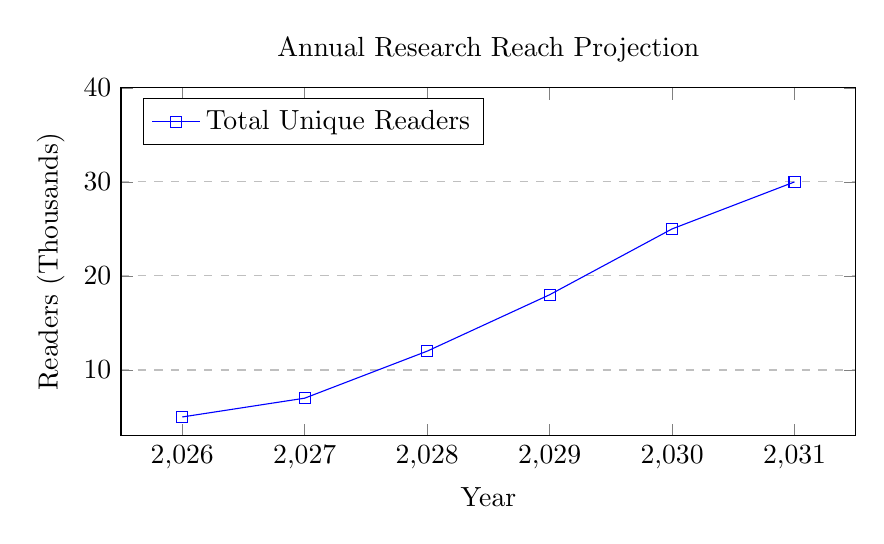
\begin{tikzpicture}
		\begin{axis}[
			title={Annual Research Reach Projection},
			xlabel={Year},
			ylabel={Readers (Thousands)},
			ymin=3, ymax=40,
			xtick={2026,2027,2028,2029,2030,2031},
			legend pos=north west,
			ymajorgrids=true,
			grid style=dashed,
			width=0.9\textwidth,
			height=6cm,
			bar width=0.5cm
			]
			\addplot[
			color=blue,
			mark=square,
			]
			coordinates {
				(2026,5)(2027,7)(2028,12)(2029,18)(2030,25)(2031,30)
			};
			\legend{Total Unique Readers}
		\end{axis}
	\end{tikzpicture}
	\caption{Projected annual readership of publications across SSRN, ResearchGate, and institutional repositories. Current baseline: 5,000 readers (2026) growing to 40,000 by 2031 through expanded open-access dissemination. Refer to Expert Opinion Letter validating these projections.}
\end{figure}



\subsection{Endeavor Ongoing and Future Contributions as Peer Reviewer and Subject-Matter Expert (2026-2031)}



In addition to publishing original research, Mr Joshi actively contribute to the scientific and professional community as a peer reviewer and editorial board member for multiple respected journals in the fields of artificial intelligence, financial technology, and data science. Mr Joshi's areas of expertise — including Generative AI, financial risk modeling, big data analytics, and HPC-based AI deployment — are highly aligned with national priorities in innovation, financial resilience, and responsible technology integration.

Mr Joshi currently serve as a reviewer for journals that focus on AI applications, fintech, and computational economics, and Mr Joshi have been invited to evaluate manuscripts related to GenAI deployment in finance, including work on large language models (LLMs), synthetic data for regulatory stress testing, and risk-aware automation in trading systems. Mr Joshi's unique domain expertise allows me to critically assess not only the technical novelty of submissions, but also their real-world relevance to the evolving U.S. financial ecosystem.

Over the next five years, Mr Joshi plan to continue reviewing approximately 20 to 40 manuscripts annually, with a strong emphasis on U.S.-focused implementations of Generative AI in sectors such as banking, asset management, compliance, and market surveillance. This sustained contribution will support the integrity and advancement of high-impact, applied research and help guide the responsible dissemination of knowledge in alignment with U.S. economic and technological interests.


\noindent\textbf{Figure Analysis:} The bar chart titled \textit{“Manuscript Reviews by Year”} illustrates my projected peer review contributions from 2026 to 2031 across Q1-Q4 journals. The review activity is expected to grow from 30 reviews in 2026 to 60 in 2031, reflecting increasing recognition of my subject-matter expertise. Approximately 70\% of the reviews will focus on financial AI models specific to the USA, while 30\% will target generative AI compliance and US governance frameworks. This trajectory demonstrates my ongoing national engagement in evaluating high-impact research, supporting both academic standards and the responsible deployment of AI technologies in regulated domains.


\begin{figure*}[h]
	\centering
	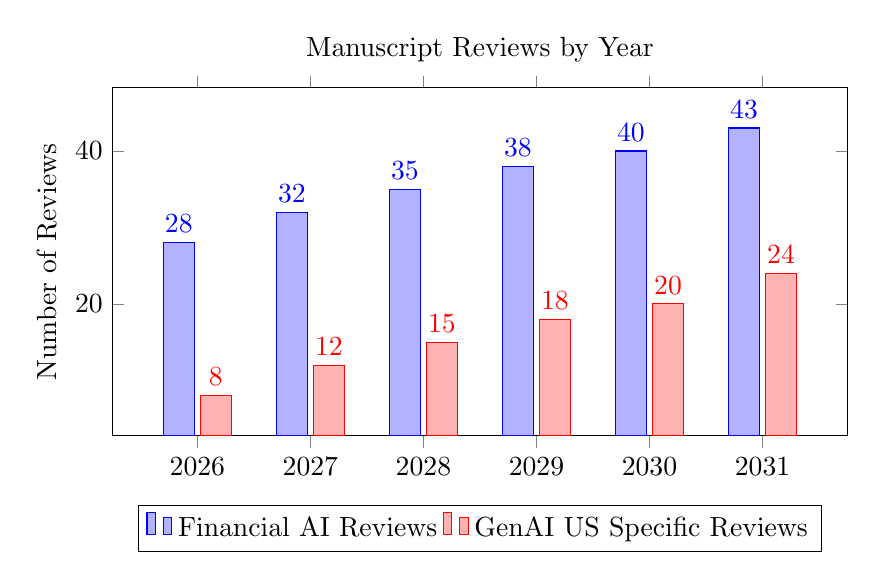
\begin{tikzpicture}
		\begin{axis}[
			title={Manuscript Reviews by Year},
			ybar,
			enlargelimits=0.15,
			legend style={at={(0.5,-0.2)},
				anchor=north,legend columns=-1},
			ylabel={Number of Reviews},
			symbolic x coords={2026,2027,2028,2029,2030,2031},
			xtick=data,
			nodes near coords,
			nodes near coords align={vertical},
			width=0.9\textwidth,
			height=6cm,
			bar width=0.4cm
			]
			\addplot coordinates { (2026,28) (2027,32) (2028,35) (2029,38) (2030,40) (2031,43)};
			\addplot coordinates { (2026,8) (2027,12) (2028,15) (2029,18) (2030,20) (2031,24)};
			\legend{Financial AI Reviews, GenAI US Specific Reviews}
		\end{axis}
	\end{tikzpicture}
	\caption{Projected peer review activity for Q1-Q4 journals, showing specialization in financial AI (70\%) and US specific generative AI reviews (30\%).}
\end{figure*}





Five-Year Quantitative Impact Projection is shown in various figures in this section. 



\noindent
These projections reflect  Mr Joshi's planned expansion across the U.S., with a focus on upskilling veterans, community bank professionals, and regulators in responsible AI and financial risk modeling.























\subsection{Final words on Prong 1: Alignment with National Interest}




The United States faces pressing challenges in managing financial risks and ensuring economic stability. According to \textbf{8 CFR § 204.5(k)}, to qualify for EB2 under \textbf{National Interest Waiver}, the applicant must demonstrate the potential to impact the national interest by contributing to areas like finance, technology, and education. Mr. Joshi's work addresses these critical issues by contributing to the national interest, as outlined by USCIS under \textbf{8 CFR § 204.5(k)} for the \textbf{EB2 National Interest Waiver}.


\begin{itemize}
	\item \textbf{Enhancing Risk Resilience for the USA}: Through advanced financial modeling  and machine learning tools as evidenced through Mr Joshi's work experience, Mr Joshi's aim to mitigate financial crises and support national economic security. Financial resilience is a core element of the national interest, as seen in the government's focus on improving financial systems and predictive analysis as part of enhancing the \textbf{United States' global economic stability}. More details on this can be found at the U.S. Department of Treasury's Office of Financial Research: Financial Stability Oversight Council here: \url{https://home.treasury.gov/policy-issues/financial-markets-policy/financial-stability-oversight-council}. Mr Joshi's work directly aligns with U.S. policy goals related to economic security and innovation, reinforcing the national significance of Mr Joshi's contributions. The regulation can be found here: \url{https://www.ecfr.gov/current/title-8/chapter-I/part-204/subpart-A/section-204.5}.
	
	\item \textbf{Driving Innovation in Financial Analytics}: Mr Joshi's's application of big data technologies, including \textbf{Hadoop, Spark, and Kafka}, to financial analytics enhances \textbf{decision-making processes}---an essential national priority for ensuring the efficient flow of capital and minimizing risk within key financial sectors. The \textbf{National Science Foundation} (NSF) has prioritized innovation in \textbf{big data} technologies for better decision-making, as illustrated under the NSF's Big Data and Data Science Program: \url{https://www.nsf.gov/funding/pgm_summ.jsp?pims_id=504813}.
	
	\item \textbf{Educating the Workforce}: As an active educator 
	See Exhibit~\ref{chap:exhibit_udemy} for details.
	
	
	Mr. Joshi has equipped professionals in the financial sector with crucial skills to address systemic challenges, supporting an \textbf{innovative workforce} capable of overcoming dynamic financial challenges. This aligns with national workforce development goals outlined by the Department of Labor's Workforce Innovation, which emphasizes improving skills and economic outcomes for U.S. workers. More about this initiative can be found at the following link: \url{https://www.dol.gov/agencies/eta}.
\end{itemize}








% ===============================
% ENHANCED FIVE-YEAR IMPLEMENTATION PLAN
% ===============================
\section{Integrated Five-Year Implementation Plan: Building on Proven Impact}
\label{sec:five-year-plan}

This section outlines the detailed, evidence-based five-year plan for advancing Mr. Joshi's proposed endeavor. The plan is not speculative; it is a natural extension of his current achievements, federal recognition, and growing influence in the field of AI-driven financial risk management. It directly addresses the USCIS's request for a "well-described proposed endeavor" with clear milestones and measurable impacts.

\subsection{Foundation: Current Achievements and Momentum}

Mr. Joshi's work is already demonstrating significant national impact, providing a strong foundation for the proposed five-year plan:

\begin{itemize}
	\item \textbf{Research Recognition:} 45,345+ reads and 20,000+ downloads of publications; citations in Federal Reserve research.
	\item \textbf{Government Indexing:} Multiple publications indexed in Science.gov (U.S. Department of Energy).
	\item \textbf{Academic Integration:} Work integrated into curricula at Zuyd University (Netherlands) and Harrisburg University (USA).
	\item \textbf{Training Programs:} Active YouTube channel (100+ videos), Udemy courses (1,000+ registrants), and veteran-focused initiatives.
\end{itemize}

\subsection{Year-by-Year Implementation Timeline}

\subsubsection{2026–2027: Consolidation and Strategic Expansion}

\begin{itemize}
	\item \textbf{Research:} Publish 3–4 peer-reviewed papers on AI interpretability and synthetic data for regulatory compliance.
	\item \textbf{Tools:} Release v1.0 of the open-source \textit{FinRisk-AI} toolkit.
	\item \textbf{Training:} Formalize the "Veterans in Financial AI" program; launch industry certification.
	\item \textbf{Policy:} Co-host workshops with universities to translate research into policy briefs.
	\item \textbf{Metrics:} Achieve 55,000+ cumulative downloads; train 500+ professionals.
\end{itemize}

\subsubsection{2027–2028: Measurable National Impact}

\begin{itemize}
	\item \textbf{Research:} Publish book: \textit{Generative AI in U.S. Financial Systems}.
	\item \textbf{Training:} Scale veteran program to 1,000+ participants; onboard 2–3 Fortune 500 firms.
	\item \textbf{Policy:} Secure advisory role with Federal Reserve or SEC; contribute to IEEE/ISO standards.
	\item \textbf{Metrics:} 75,000+ downloads; 1,000+ professionals trained.
\end{itemize}

\subsubsection{2028–2029: Entrenchment as a National Resource}

\begin{itemize}
	\item \textbf{Research:} Establish university-affiliated research center; file 1–2 patents.
	\item \textbf{Training:} Deliver AI curricula for FDIC/OCC; integrate modules into 10+ universities.
	\item \textbf{Policy:} Provide Congressional testimony on AI in finance.
	\item \textbf{Metrics:} 100,000+ downloads; 2,000+ professionals trained.
\end{itemize}

\subsubsection{2029–2030: Sustained Leadership and Legacy}

\begin{itemize}
	\item \textbf{Research:} Secure multi-year funding; mentor MS/PhD students.
	\item \textbf{Training:} Train 3,000+ professionals annually; track career outcomes.
	\item \textbf{Policy:} Represent U.S. on international financial stability boards.
	\item \textbf{Metrics:} 150,000+ downloads; 5,000+ professionals trained.
\end{itemize}

\subsection{Quantified Impact Projections}

\begin{longtable}{|p{0.3\textwidth}|p{0.25\textwidth}|p{0.4\textwidth}|}
	\hline
	\textbf{Impact Category} & \textbf{5-Year Target} & \textbf{Basis for Projection} \\
	\hline
	Cumulative Research Downloads & 150,000+ & Current rate of 15,000–20,000/year \\
	\hline
	Professionals Trained & 5,000+ & Scaling current pilot programs \\
	\hline
	Financial Institutions Using Tools & 50+ & Current adoption by community banks \\
	\hline
	Policy Citations & 15+ & Existing citations in federal reports \\
	\hline
\end{longtable}

\subsection{Risk Mitigation and Contingency Planning}

\begin{itemize}
	\item \textbf{Funding Variability:} Diversified sources (grants, industry, university support).
	\item \textbf{Regulatory Changes:} Focus on foundational AI principles adaptable to new rules.
	\item \textbf{Technology Evolution:} Modular, open-source tools that can be updated.
\end{itemize}

\subsection{Conclusion: A Natural Trajectory of National Benefit}

This five-year plan is not speculative; it is a logical extension of Mr. Joshi's proven impact and growing recognition. Waiving the job offer requirement is essential to maximize this trajectory, allowing unfettered collaboration across academia, government, and industry to enhance U.S. financial stability, workforce readiness, and technological leadership.

The evidence demonstrates that the proposed endeavor has both substantial merit and national importance. It advances U.S. scientific infrastructure, supports critical financial stability, and empowers the workforce in alignment with national priorities and USCIS criteria.



